
\chapter{Enhancing human-robot physical collaboration with polytopes}


\section{Motivation: Collaborative Workstation}
The industry of the future, as described by the movement called Industry 5.0~\cite{MADDIKUNTA2022ind50}, promises to step away from the traditional point of view on industrial automation, where the goal is to blindly automatise, as much processes as possible, in order to improve the overall efficiency and reduce the cost. The Industry 5.0 puts the human workers in the central position and aims to create the workflows that ensure their well-being as well as the long term sustainability of the industrial practices in general~\cite{XU2021ind50}. The industry of the future relies on the flexibility and adaptability of the human workers, by embracing their cognitive and physical skills as well as their talents and different levels of expertise. The role of the automation is no longer purely optimisation of the industrial processes, but providing the support and assistance to the human operator with the aim to exploit both machines' and humans' full potential, establishing human-automation symbiosis~\cite{LENG2022ind50} on the industry floor.
 
One typical example of such symbiosis is an industrial workstation~\cite{SIMOES2022workplace}, where the human and the robot work in a close proximity and interact physically to execute different tasks. The aim of such collaboration is to improve the overall efficiency by exploiting the abilities of both humans (flexibility, adaptability, cognitive capacity, expertise, etc.) and robots (repeatability, precision, tirelessness, etc.), as well as to improve the operators well-being, remove the unnecessary strain and ensure his safety when executing tasks. Therefore, such future collaborative scenarios require having a set of tools for characterising different abilities of robots and humans, as well as different notions of human well-being and safety. Such tools are required both for assessing different tasks and allocating them with respect to humans and robots abilities as well as for creating more human-centred robot control strategies.

\todos{I'm more or less happy till here}

Even though human-robot collaboration is still relatively recent field, there are numerous performance metrics proposed in the literature that quantify different aspects of the quality of their collaboration and their individual abilities~\cite{CORONADO2022collab_quality}.
The main focus of this work is put on different tools for characterising human's and robot's physical abilities, especially their polytope representations, which have a great potential to be used in this context, both in order to quantify and leverage their individual abilities as well as to ensure human safety. As discussed in chapter \ref{ch:poly_metrics}, the polytope characterisations of different physical abilities are an accurate representations of physical abilities for both robots and humans. Furthermore, the polytopes enable expressing their individual physical abilities, as well as their joint physical abilities when collaborating, in the same polytope form. Such unified view on their capacities lays foundation for creating new task allocation strategies that take in consideration their physical abilities, by being able to asses if different tasks better suite human's or robot's abilities or potentially require their collaboration. 

Furthermore, both human's and robot's physical abilities are state dependant and can vary significantly during the task execution, and polytopes enable capturing the changes in their abilities as well. Having an accurate information about the robot's physical abilities online, enables creating robot control strategies that adapt to the their changes and exploit the robot's full potential. On the other hand, having an accurate online information about the human's physical abilities is important for assessing if the operator is apt to execute a certain task and quantifying if the operator needs assistance of the robot due to its lacking physical abilities. Furthermore, having the real-time information about the operator's physical abilities enables ensuring that his abilities are never surpassed which has a direct impact on the operator's safety and well-being. Therefore, the collaborative workstations require creating more human-centred robot control strategies where the robot adapts its behaviour not just with respect to the requirements of the task and its own abilities, but also to the current abilities of the human operator as well as his safety. As polytope characterisations of robot's and human's physical abilities can be easily integrated with different robot control strategies, they have a great potential to be used for creating such adaptive collaboration scenarios.

\todos{more or less happy.}

This chapter present the benefits of using the polytope based physical ability characterisations for creating real-time robot control strategies that enable such flexible collaboration scenarios. Section \ref{ch:collaborative_carrying} brings an example of the task of collaborative object carrying within the collaborative workstation, where two collaborative scenarios are proposed. First scenario, introduced in section \ref{ch:robot_robot_carrying}, consists in two robots collaborating to carry a heavy object while the control strategies of each one of the robots take in consideration both their own and the other robot's physical abilities. Second scenario, proposed in section \ref{ch:human_robot_carrying}, consists in the human operator and the robot collaboratively carrying a heavy object, where the robot's control strategy takes in consideration its own physical abilities and the physical abilities of the operator in the real-time. 

\todos{
Furthermore, an assistive and human-centred robot control strategy that exploits the polytope geometry is described in section after.
}

\section{Collaborative carrying of a heavy object}
\label{ch:collaborative_carrying}

\begin{figure}[!h]
    \centering
    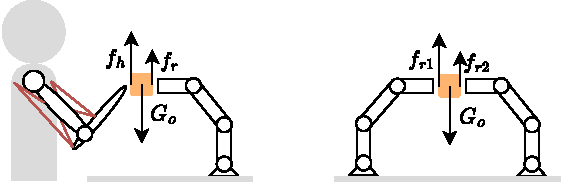
\includegraphics[width=0.6\linewidth]{Papers/images/carrying_schema.pdf}
    \caption{}
    \label{fig:carrying_schema}
\end{figure}

One traditional example of a collaborative task requiring physical interaction between multiple actors (humans and robots) is collaborative object carrying~\cite{Arai2000carrying,Kosuge1997carrying,Tsumugiwa2002carrying}. In this task $N$ actors collaborate physically by applying forces $\bm{f}_{a_i}$ on the object with mass $m_o$, in order to compensate for its gravity $G$
\begin{equation}
    G=m_o\bm{g}=\bm{f}_{a_1} + ~\cdots ~+\bm{f}_{a_N}
\end{equation}
An illustration of the human-robot and dual robot arm collaborative carrying is given on Figure \ref{fig:carrying_schema}. 



\todos{
\begin{itemize}
    \item each one of the actors has a certain capacity to carry the objects
    \item their common capacity is the some of the two
\end{itemize}
}

% \begin{figure}[!h]
%     \centering
%     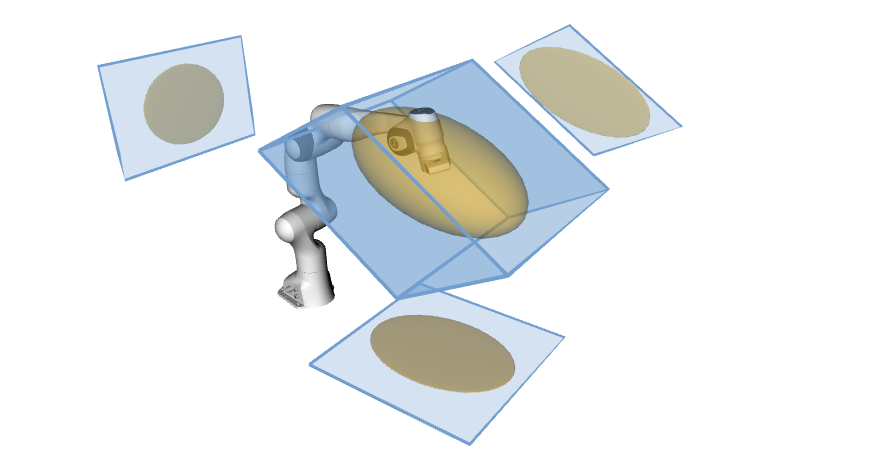
\includegraphics[width=0.5\linewidth]{Papers/images/polytope_ellipsoid.png}
%     \caption{}
%     \label{fig:panda_polytopes}
% \end{figure}

% \begin{figure}[!h]
%     \centering
%     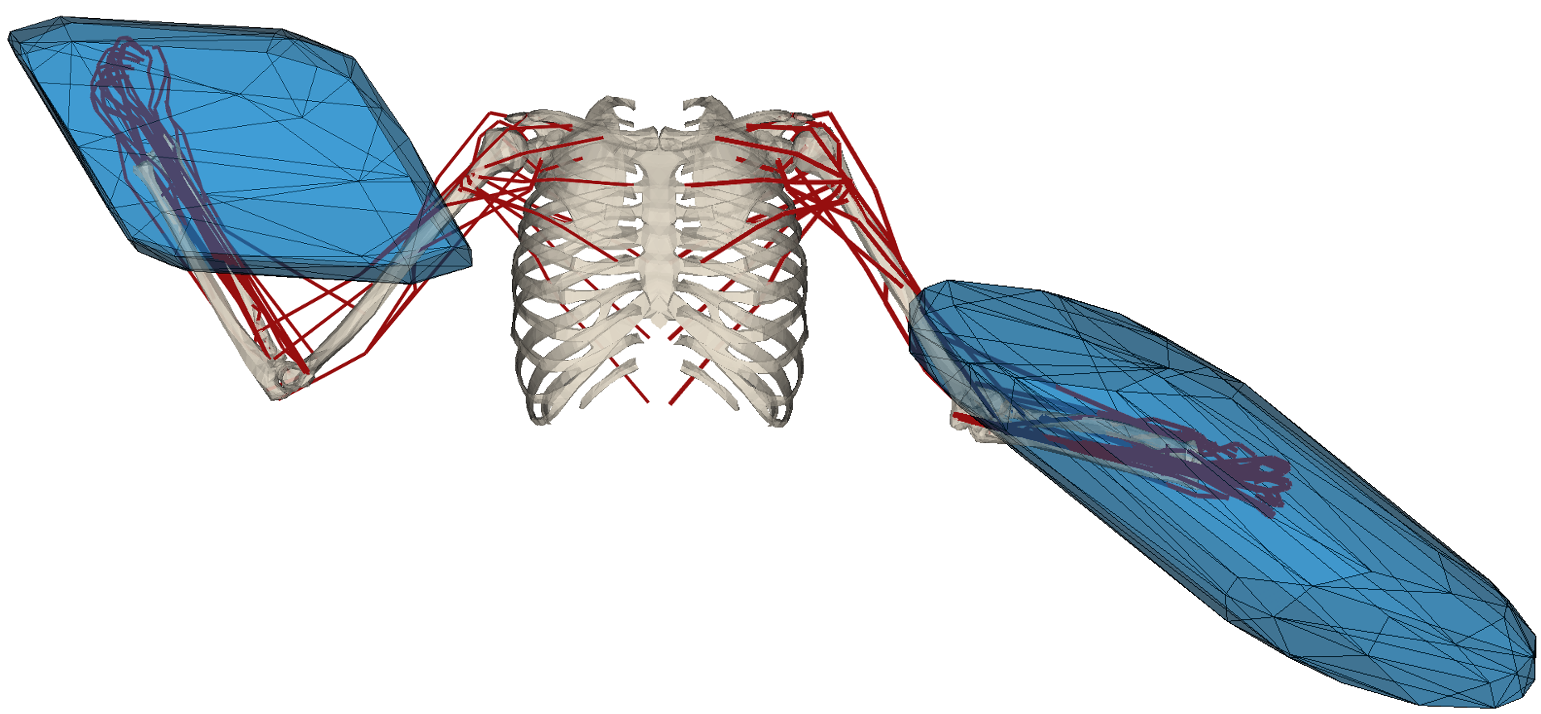
\includegraphics[width=0.5\linewidth]{Papers/images/bimanual.png}
%     \caption{}
%     \label{fig:images_bimanual}
% \end{figure}

\subsection{Dual robotic arm collaborative object carrying}\label{ch:robot_robot_carrying}


\subsubsection{Robot carrying capacity calculation}

\begin{figure}[!h]
    \centering
    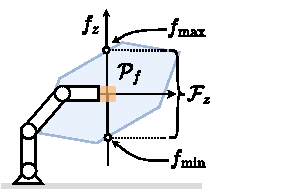
\includegraphics[width=0.4\linewidth]{Papers/images/carrying_capacity_robot.pdf}
    \caption{}
    \label{fig:collaboartion_schema}
\end{figure}

\todos{
\begin{itemize}
    \item Carrying capacity can be calculated for robots as their wrench capacity
    \item then their polytope can be intersected with $z$ axis
\end{itemize}
}

\subsubsection{Robot control experiment}

\begin{figure}[!h]
    \centering
    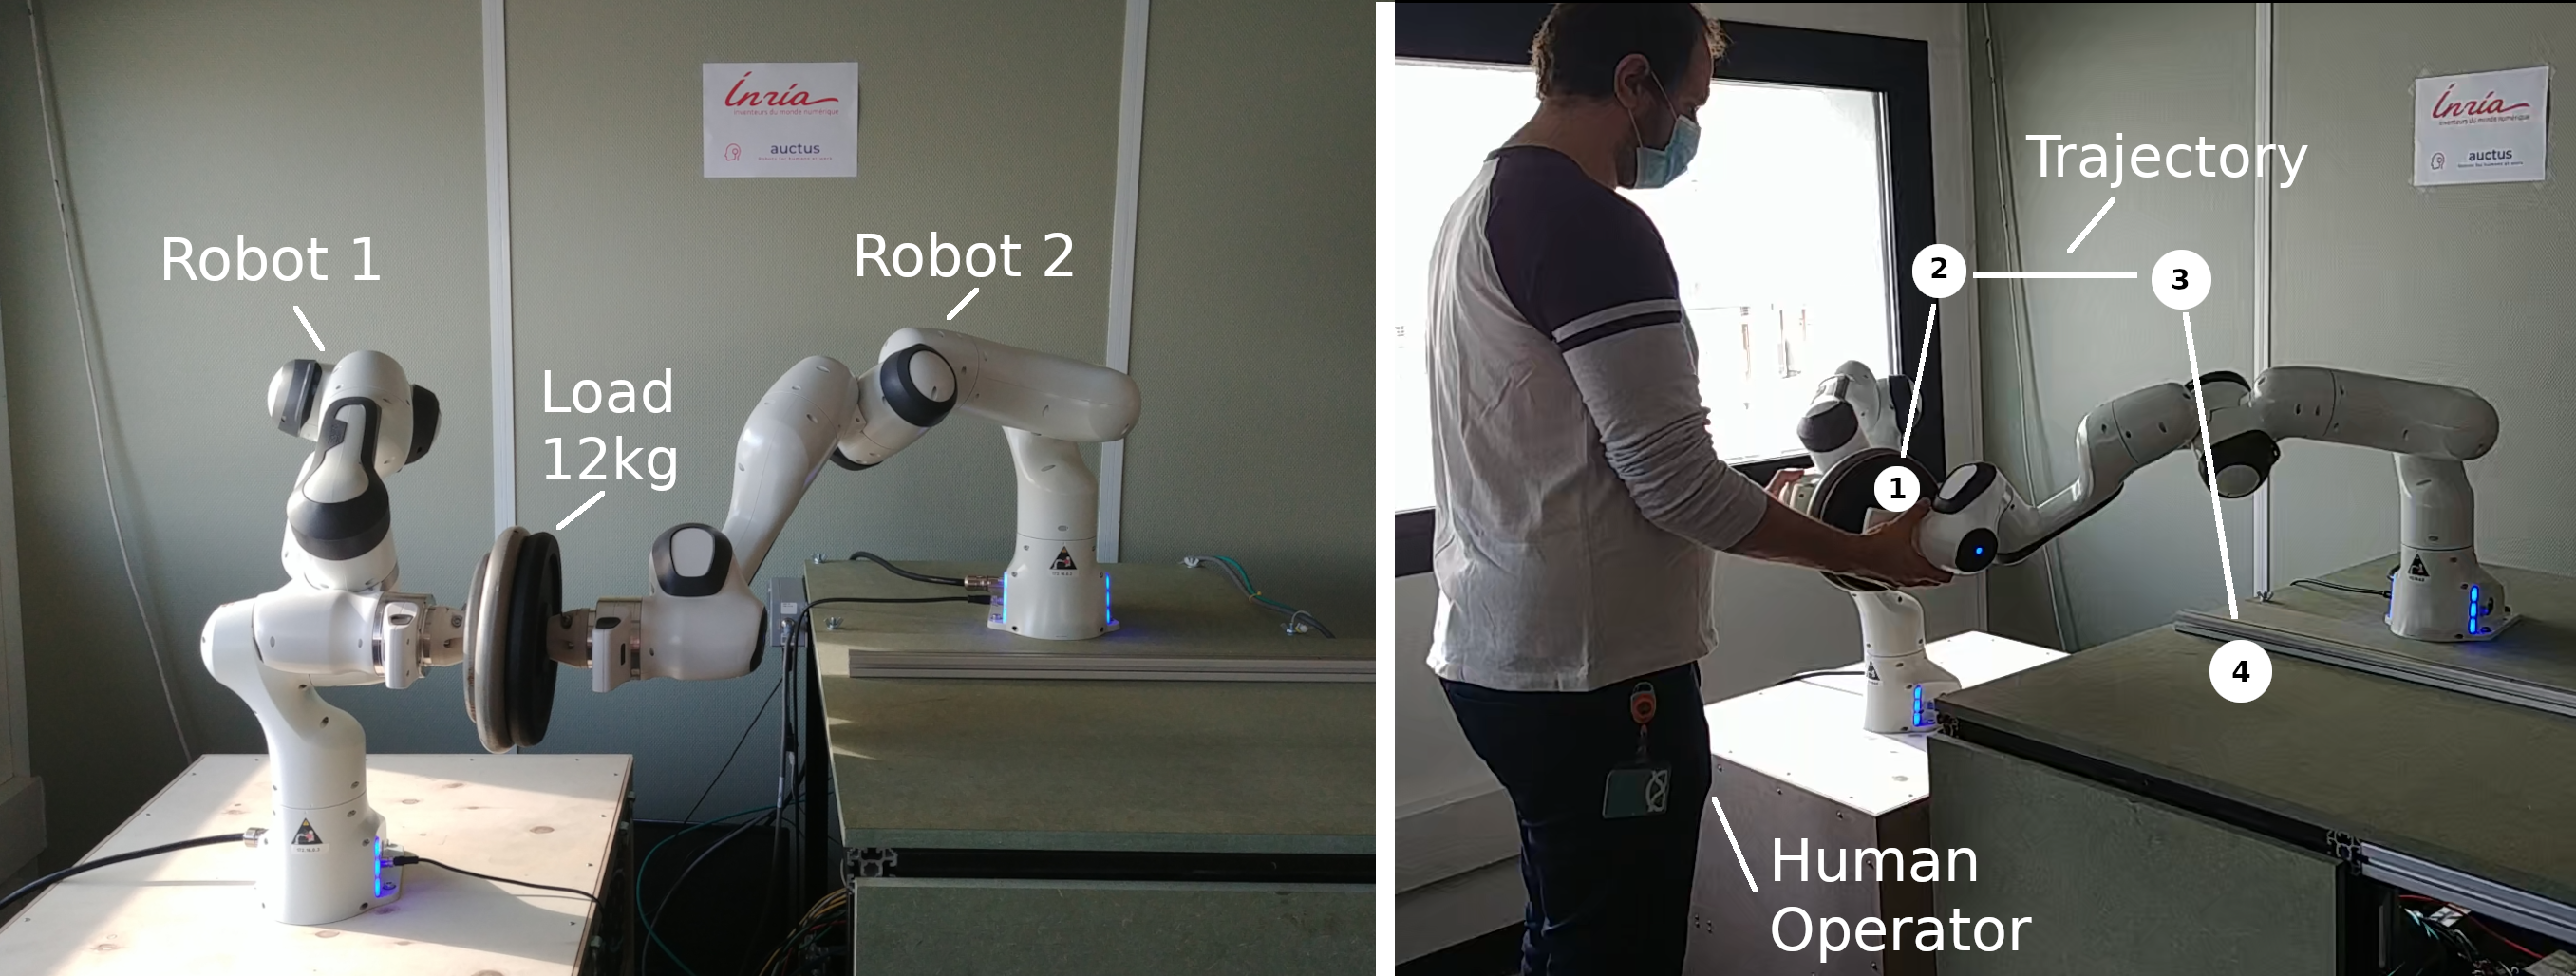
\includegraphics[width=\linewidth]{Papers/images/exp1_explication.png}
    \caption{}
    \label{fig:experiment1}
\end{figure}


In this section, the real-time force capability evaluation is employed in the context of robot control. An experiment is designed using two \textit{Franka Emika Panda} robots involved in a collaborative load carrying task for an object of mass $M$. Each robot is contributing to the compensation of the overall gravity force $G=Mg$ applied at the end-effector by the carried object, with forces $f_1$ and $f_2$ respectively such that
\begin{equation}
    f_1 + f_2 = G
\end{equation}
Additionally, a human operator is moving the object freely through the common work-space, implicitly changing both robots positions and configurations in real-time. As a consequence, the task space trajectory and the evolution of the robot configurations are not known in advance.

The experiment has been implemented using the ROS programming environment. Both robots are torque controlled at $1 kHz$. The update of the force capability estimation are performed at 40$Hz$. All the control software is run from one computer with the 1.90GHz Intel i7-8650U processor. This experiment is illustrated in the accompanying video.

Panda robots are rated to a maximal carrying capacity of 3kg which corresponds to the absolute minimal carrying capacity of the robot evaluated in one of its near-singular configurations. It is, by definition, an underestimation of the real robot task space wrench capacity and relying on it, as it is commonly done, limits the scope of the possible tasks and applications.

The goal of this experiment, it is to demonstrate the fact that, taking into account the true force capabilities of each robot, it is possible to considerably go beyond the robots conservative rated capacity without comprising safety nor exceeding any of the actuation limits. The weight of the object chosen for the experiments is $M=12kg$, voluntarily far above the recommended joint carrying capacity $M \le 6kg$. 

\begin{figure}
    \centering
    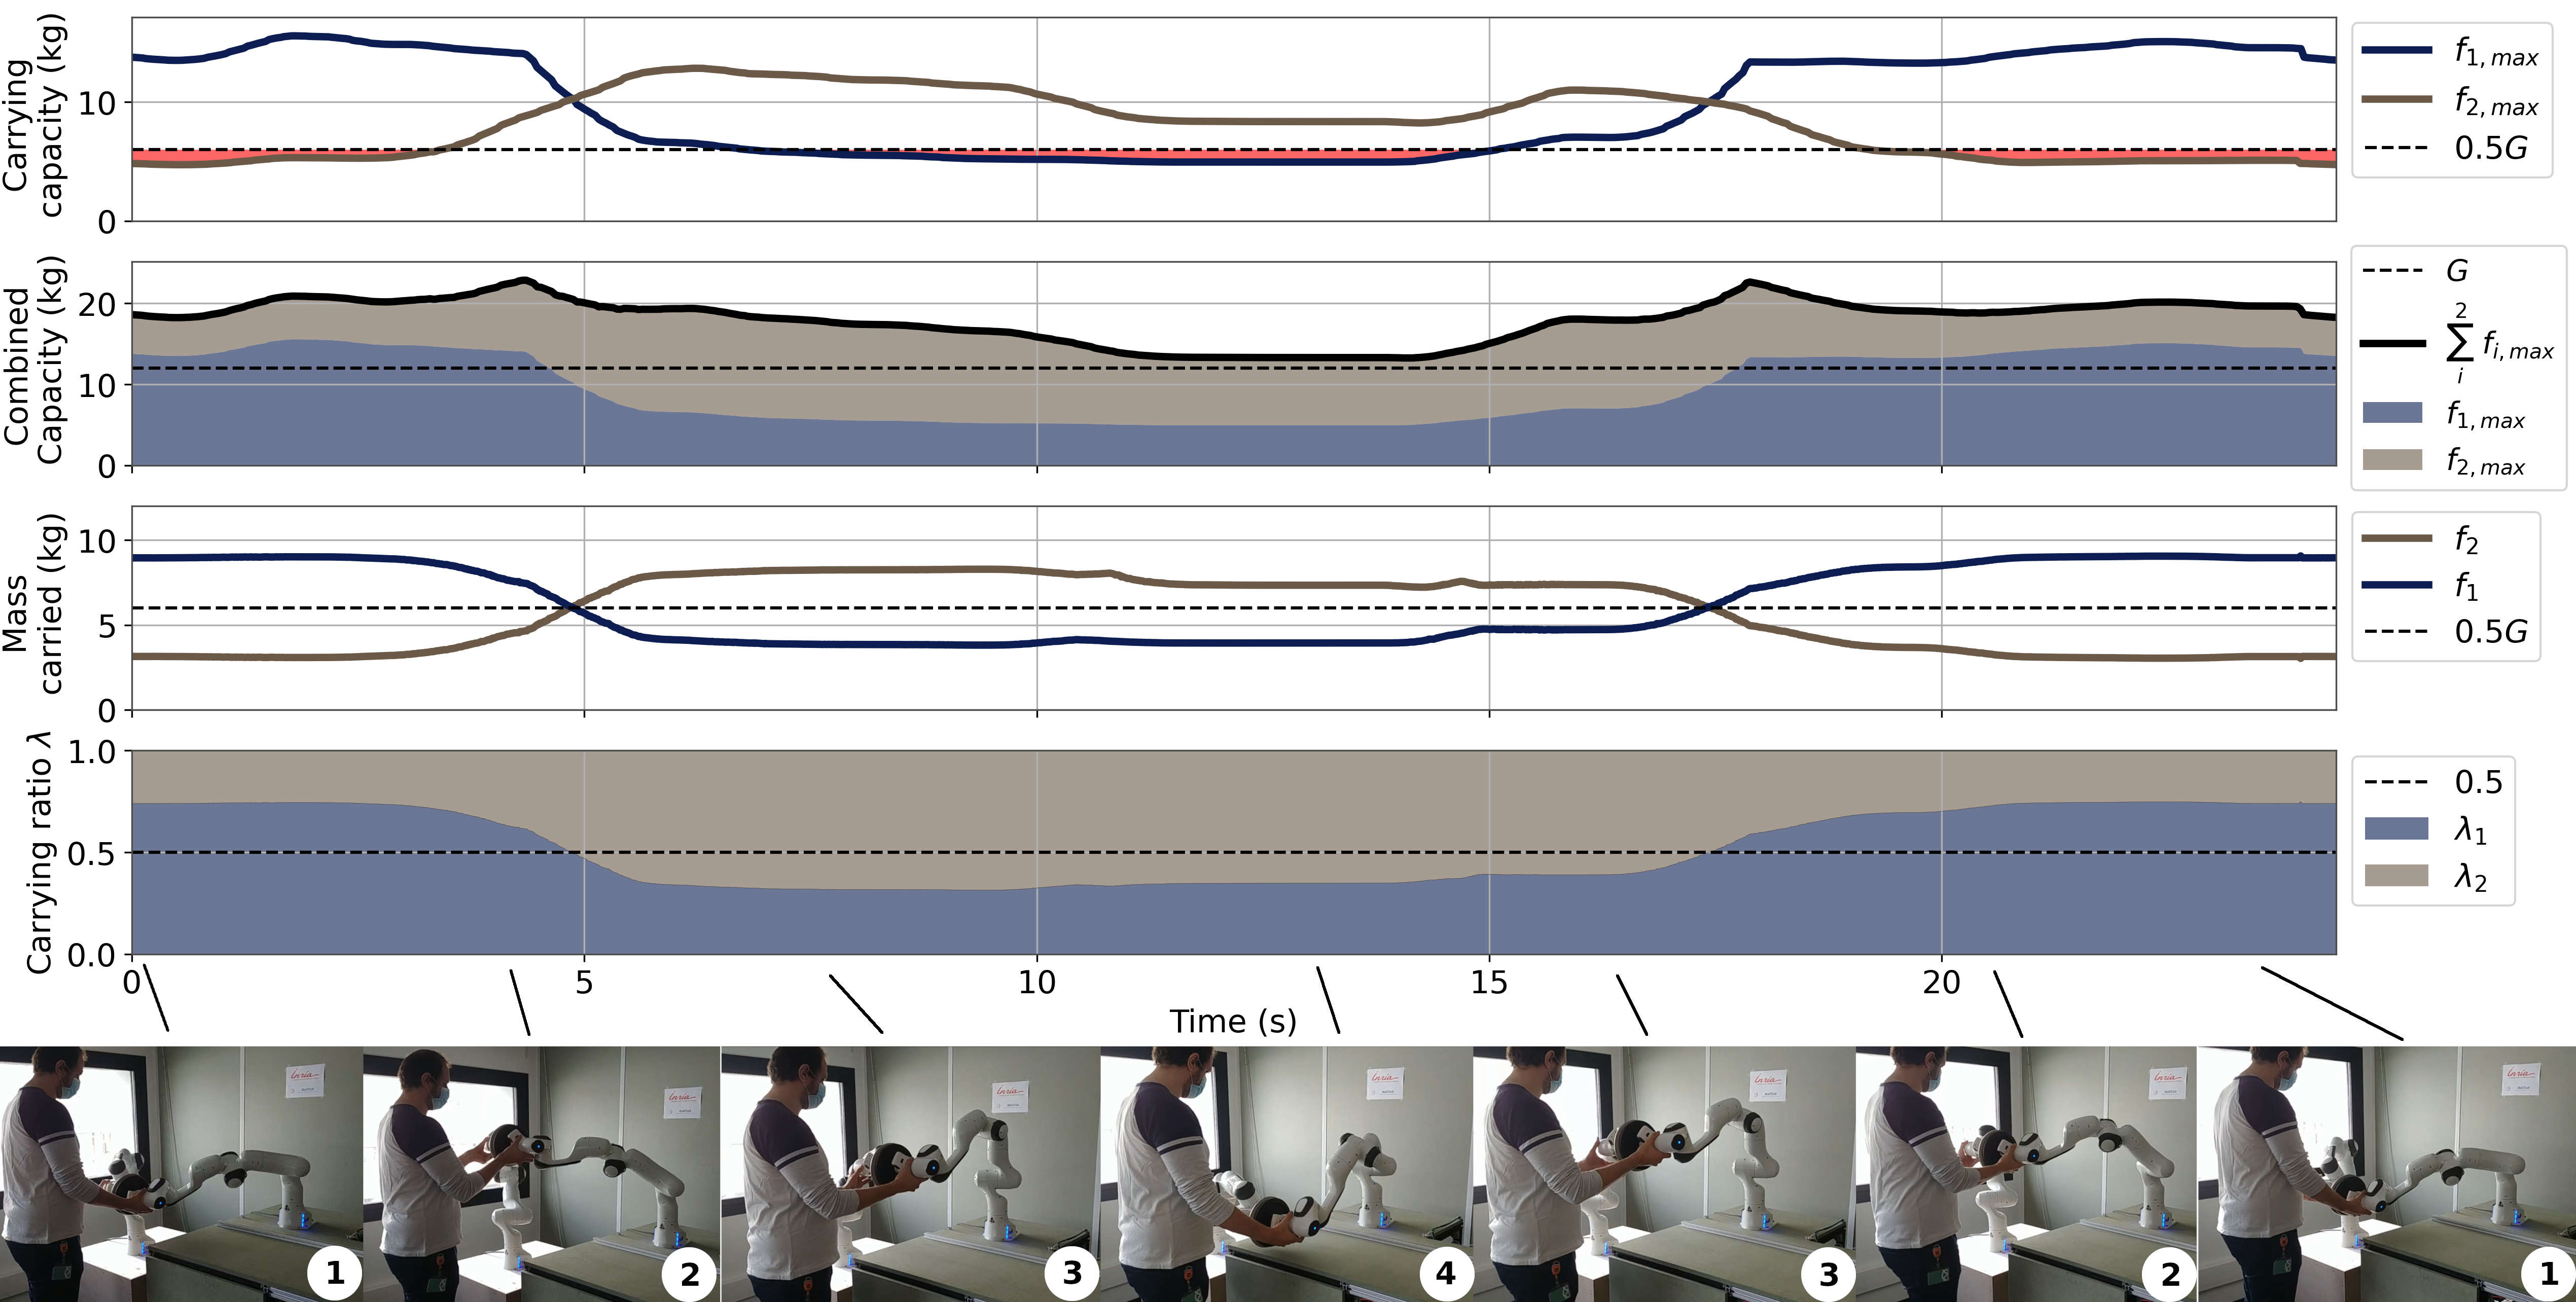
\includegraphics[width=\linewidth]{Papers/images/exp_no_anim.jpg}
    \caption{Images 1 to 4 on the right show the sequence of poses the manipulators are placed by a human operator during the course of the experiment. On left side, on the top is the graph showing the time evolution of applied manipulator forces $f_1,f_2$. The middle graph provides the evolution of the maximal applicable forces $f_{i,max}$ of each manipulator separately and their joint capacity $F_{max}$, based on the proposed polytope evaluation algorithm. In this graph,  the time periods when the constant strategy $\lambda$=$0.5$ (dashed line on all graphs) would not be feasible for at least one of the two robot are indicated with red background. The bottom graph shows the  evolution in time of the control parameter $\lambda$ for the proposed adaptive strategy.}
    \label{fig:dual_manip}
\end{figure}


Evaluating the maximal applicable force in the vertical direction can be viewed as a special case of the force polytope $\mathcal{P}_f$ vertex search problem where the task-space force of interest $f$ is a scalar and $m=1$.
The proposed algorithm described in section \ref{sec:algorithm} is used to efficiently find $f_{i,max}$, the limits (vertices) of the maximal applicable force in $z$-axis direction, for each robot separately.  Their overall carrying capacity can be calculated as the sum of the two $F_{max} = f_{1,max} + f_{2,max}$.

To efficiently distribute and adapt the carried load in between robots, each robot compensate for a part of the object's weight $G$ which is proportional to its force capacity  $f_{i,max}$  
\begin{equation}
   f_1 = \lambda G \quad f_2 = (1-\lambda)G,\quad \lambda = \frac{f_{1,max}}{f_{1,max} + f_{2,max}}
\end{equation}
 
A straightforward control strategy, requiring each robot to compensate for half of object mass $f_1=f_2=0.5G$ is taken as baseline to evaluate the performance of the new method.

Figure \ref{fig:dual_manip} (right) shows one possible manipulation trajectory, where a human operator displaces the carried object in the common workspace in four discrete locations over a 20 seconds period of time. On the left side of the figure \ref{fig:dual_manip} the evaluated maximal forces and force applied by each robot during the experiment are shown. Additionally, the $0.5G$ strategy line is shown for comparison. 

The proposed control strategy is successful in ensuring  compensation of the object weight during the full length of the experiment. In the starting pose $t=0s$, robot 2 (robot on the left) is close to it's singular configuration and its load carrying capacity is close to 5kg. Controlling it to compensate for half of the weight of the object would result in a security exception and could damage the robot hardware. The same is true for pose 4 at $t=17s$. Robot 1 (robot on the right) is not be able to compensate for half of the object weight but thanks to the proposed adaptive control law, the task can successfully be achieved. This may not be the case over the entire common workspace of the two robots but this example is a good illustration of the interest of accounting for the true capabilities of the system at the control level.  An additional interesting result from the experiment is the transition between pose 3 and 4 ($t \in [12s,16s]$). Even though the object is much closer to robot 2 (right), robot 1 has a much higher carrying capacity. This illustrates the fact that force capabilities are highly nonlinear functions which are very hard to predict. This provides an additional argument in favor of on-line force capacity evaluation. 

\begin{equation}
\begin{split}
    \min_{f_1,f_2} &~||G - f_1 -f_2||^2 ~~+ \omega\lambda||f_1||^2 + \omega(1-\lambda)||f_2||^2\\
    s.t.& \quad f_1 \in[0, f_{1,max}]\\
    & \quad f_2 \in[0, f_{2,max}]\\
\end{split}
\end{equation}


\subsection{Human-robot collaborative object carrying}
\label{ch:human_robot_carrying}


\todos{
\begin{itemize}
    \item Naive approach for human-robot collaboration is for the robot to carry everything
    \item human power applied is studied \cite{Mujica2020Evaluation}, ergonomic indicators (REBA) \cite{ferraguti2020unified},  static joint overloading \cite{Kim2018}
    \item First this is not always possible, robot's carrying capacity is limited and it might require buying a huge robot which would not be safe to the operator any more
    \item second the studies have shown that human's engagement to the task is proportional to the level of the physical effort exerted
    \item Exoskeletons \cite{petric2019assistive}, \cite{carmichael2013admittance}
    \item once when we've decided to separate the weight, how do we do that?
\end{itemize}
}

\subsubsection{Human carrying capacity calculation}
\begin{figure}[!h]
    \centering
    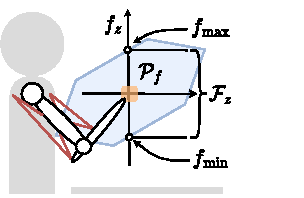
\includegraphics[width=0.4\linewidth]{Papers/images/carrying_capacity_human.pdf}
    \caption{}
    \label{fig:collaboartion_schema}
\end{figure}

\todos{
\begin{itemize}
    \item Carrying capacity can be calculated for robots as their wrench capacity
    \item then their polytope can be intersected with $z$ axis
\end{itemize}
}

\subsubsection{Robot control experiment}

%To illustrate the potential of the proposed algorithm for the human-centered robot control, a mockup load carrying experiment is conducted. 
An example experiment is conducted, designed as a simplified heavy object manipulation task common in the industrial assembly procedures. 

In the experiment, shown in the figure \ref{fig:experiment}, a human operator and a \textit{Franka Emika Panda} robot jointly carry $m_o\!=\!7$ kg object, each one compensating for a part of the total weight {$ f_h\! +\! f_r\! =\! m_og\! =\! G_o $}. The human operator {visually} navigates the object through the common workspace, passing through {the set of} 4 via-points. 
{The experiment is repeated two times, 
for two different operator positions, equally distant from the via-points, but rotated by 90° in space.}

\antun{
Naive gravity compensation strategy would be the usual choice for these experiments, making the robot carry the full weight of the object and provide the operator with full movement transparency. However, several studies have shown that the human's physical feedback during task execution improves significantly his engagement in the task \cite{rani2007operator}, improves the task execution efficiency and reduces the risk of the human error \cite{BYRNE1996249}. 
Since the human's carrying capacity varies significantly throughout the workspace, allocating any fixed weight to the operator requires \textit{a priori} analysis of the task and determination of the, often conservative, \textit{"worst-case"} weight limits \cite{shoaf1997comprehensive}\cite{health1992manual}, often highly specific to the task in question.  
} 


{As the human operator's carrying capacity can be expressed as the maximal force the operator's arm can generate in the $z$-axis (vertical) direction, proposed CHM algorithm can be used to calculate it in real-time.}
% \antun{  As the proposed CHM method can be used to calculate operator's carrying capacity in real-time, as the maximal force the operator's arm can generate in the $z$-axis (vertical) direction, 
{ Inspired by} the \textit{Assist-As-Needed} (AAN)\cite{carmichael2013admittance} paradigm, {a simple adaptive weight distribution strategy is designed, with goal to ensure} that the human operator's relative load remains constant with respect to its real-time capacity. The fixed ratio chosen for the experiments is 30\% of the human's carrying capacity, {ensuring operator's safety and maintaining the constant level of engagement}.
$$
f_h = 0.3 f_{h,max}, \quad f_r = G_o - f_h
$$


\begin{figure}[!t]
    \centering
    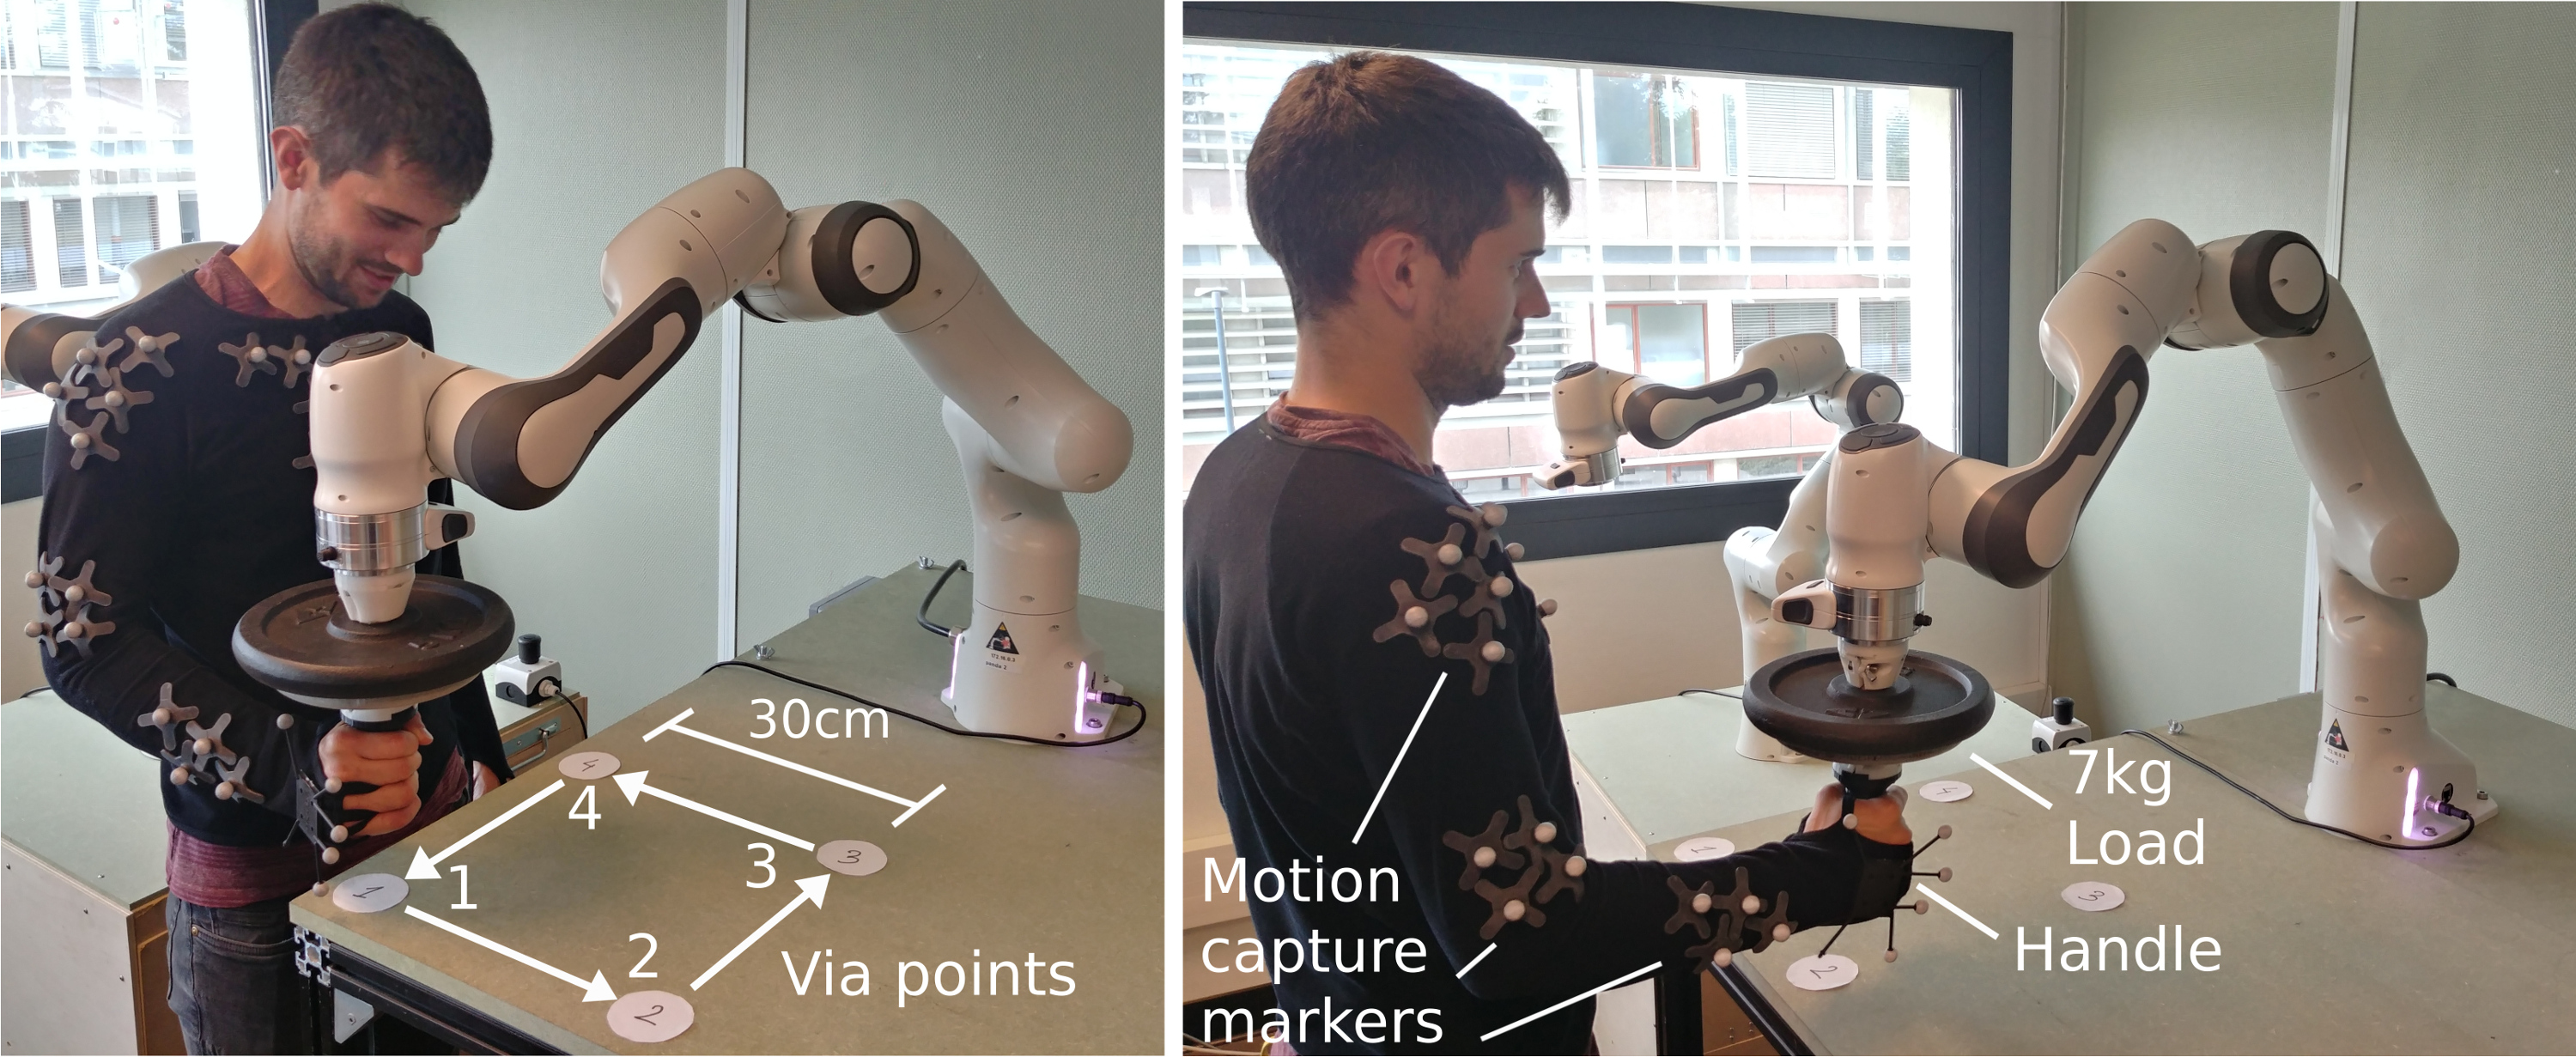
\includegraphics[width=\linewidth]{Papers/images/both_pose_explanation.jpg}
    \caption{{These figures show the experimental setup. The robot end-effector is fixed to the carried object and the human operator is holding the object by the handle. The motion capture system is used to acquire the pose of the human arm. The via-points are visually indicated to the human operator with numbered stickers on the table placed at the corners of a 30 cm square. The images shows the experiment 1 (left) and the experiment 2 (rigth).}}
    \label{fig:experiment}
\end{figure}

The human upper limb configuration is inferred in real-time using an \textit{Optitrack} motion capture system. The musculoskeletal model analysis is developed using the efficient C++ library \textit{pyomeca biorbd} \cite{Michaud2021}. The musculoskemetal model used in this experiment is the 50 muscles, 7 degrees of freedom MOBL-ARMS model \cite{saul2015benchmarking}  {developed by Holzbaur et al. \cite{holzbaur2005model}. The human subject (male, 182 cm, 80 kg) and the model belong to the same 50th percentile anthropomorphic group \cite{gordon1989anthropometric} so no model scaling \cite{correa20112782} is necessary.}

The robot is controlled using the direct force control
$$
\bm{\tau}_r = J_{ee}^T(\bm{q}) f_r + \bm{\tau}_{g,r}(\bm{q})
$$
where $J_{ee}$ is the end-effector Jacobian, $\bm{\tau}_{g,r}$ is robot's gravity torque vector and $\bm{\tau}_r$ are the joint torques applied to the robot. 
{The carrying capacity of the robot is calculated using the real-time algorithm} \cite{skuric:hal-02993408}, making sure that its capacity is not exceeded as well. All the algorithms are implemented in Python, integrated using the \textit{Robot operating system} (ROS) and run on a computer with 1.90GHz Intel i7-8650U processor. 

Figure \ref{fig:experiment_results} confirms that the evolution of robot's carrying capacity does not change in both experiments, as the via-points' position remains fixed, {whereas human's carrying capacity profile changes significantly}. The human's carrying capacity in both experiments peaks around 20 kg demonstrating that the human's force capacity is not negligible with respect to the robot's, however its large variability, from 20 kg to less than 5 kg, emphasizes the importance of measuring it in real-time.    

Figure \ref{fig:experiment_results} further shows that, by calculating the operator's carrying capacity in real-time, { using the same simple control law, the robot is able to adapt its assistance strategy despite the substantial change in the operator's capacity profile.}
To demonstrate this adaptability even further, in addition to  experiments 1 and 2 , a third experiment is included in the video attachment, where the human operator moves freely in space. 

\begin{equation}
\begin{split}
    \min_{f_r,f_h} &~||G - f_r -f_h||^2 ~~+ \omega||f_r||^2 - \omega f_h\\
    s.t.& \quad f_h \in[0, ~f_{h,max}]\\
    & \quad f_r \in[0, ~f_{r,max}]\\
\end{split}
\end{equation}


\begin{figure}[!t]
    \centering
    \includegraphics[width=\linewidth]{Papers/images/exp2_no_anim.png}
    \caption{This figure shows the evolution of the carrying capacity and weight carried by the operator and the robot over the course of the via-point cycle, for two experiments. The plots show mean values and the variances of the curves calculated over 10 successive cycles. The graph regions belonging to the different via-points are separated by vertical lines.  All the values are expressed in kilograms for easier readability.}
    \label{fig:experiment_results}
\end{figure}

\subsubsection{Prospective for human-robot collaboration}
The proposed algorithm presents a new and efficient way of calculating human's wrench capabilities which, as opposed to the known methods (ellipsoids \cite{yoshikawa1985manipulability}\cite{sasaki2011vertex} or RSM algorithm \cite{carmichael2011Towards}), can guarantee user defined level of accuracy. It opens many possibilities for wider use of human wrench polytopes in the area of the human-robot collaboration, by both reducing the computation time and enabling the use of more complete human models, better describing human subjects \cite{sohn2019effects}.

Analysis based on the more complete human models and their pathology could enhance the exoskeleton and prosthesis design, while the efficiency might accelerate analysis of wider anthropomorphic groups of people and improve the design of collaborative workspaces. The algorithm's real-time ability, on the other hand, may enable higher degree of human-centered robot control. The operators' accurate real-time capacity, based on the detailed musculoskeletal models, could be used not only to enforce safety and improve engagement, but to provide the operator-specific assistance profiles. Preventing the development of the work related injuries and potentially even enabling the rehabilitation in the factory context.

Furthermore, the  also relate to the inclusion of capability alteration models related to fatigue but also cognitive factors. This potential increase in models complexity advocates for systematic experimental validations of the results they lead to \cite{biomechanics1010008}.

The potential of the method to be used for collaborative robot control is demonstrated in a collaborative carrying experiment, where the human operator and a robot jointly carry a 7kg object. The experiment shows that by combining the real-time human's capacity evaluation with a simple control law, a highly flexible collaboration scenario can be created. 

Even though the proposed algorithm itself is independent of any musculoskeletal model, it relies entirely on the model's real-time representation of the operator. Therefore, for practical implementations, the key challenges become: evaluating human posture in the real-time, precise enough and in a minimally intrusive way, as well as performing the individual scaling and calibration of the used musculoskeletal models for a given operator \cite{correa20112782}.

\section{Reachable space shaping}
\label{ch:human_robot_reachable_space}


\section{Perceived mass shaping}
\label{ch:human_robot_percieved_mass}


\section{Conclusion}

